\documentclass[a4paper,10pt]{scrartcl}
\usepackage[ngerman]{babel}
\usepackage[T1]{fontenc}
\usepackage[utf8]{inputenc}
\usepackage{float}
\usepackage{graphicx}
\usepackage{amsmath}
\usepackage{upgreek}
\title{Statistik 2018}
\author{Benjamin Altmiks}
\date{2. Oktober 2018 - \today}
\begin{document}
\maketitle
\tableofcontents
\newpage
\section{Einführung}
\begin{quote}
    „ There are three kinds of lies: lies, damned lies and statistics.“ \newline Leonard Henry Courteney
\end{quote}
\subsection{Allgemein}
Die Statistik ist aufgeteilt in die Zusammenstellung von Zahlen und die statistische Methodenlehre. Die statistische Methodenlehre beeinhaltet die Desprektive (Durchschnittliche Berechnung) und Induktive (Schätzung und Testen) Statistik sowie die Wahrscheinlichkeitstheorie.
\subsection{Merkmale}
Merkmale können als \textbf{qualitativ – quantitativ} und \newline \textbf{diskret (Abzählbar) – stetig (Nicht Abzählbar)} definiert werden. \newline
Die Grundgesamtheit ist die Menge aller relevanten Merkmalsträger
\subsection{Skalenniveaus}
Man unterscheidet Skalenniveaus zwischen: \newline\newline
\textsc{Nominalskala}: Daten die in keine logische Reihenfolge gebracht werden können wie Farben oder das Geschlecht
\newline\newline\textsc{Odinalskala}: Können in logische Reihenfolge gebracht werden, aber nicht quantifiziert werden, das heißt man kann nicht mit ihnen rechnen. Ein Beispiel hierfür sind Schulnoten
\newline\newline\textsc{Kardinalskala}: Sind Daten die in logische Reihenfolge gebarcht werden können, sowie eine Differenzbildung sinnvoll und möglich.
\subsection{Skalendegression und Skalenprogression}
Ist eine Skalierung um Informationen angemessen und möglichst genau darzustellen.\newline
\textbf{Skalendegression}: Durch Informationsverlust können alle Merkmale nominal Skaliert werden, metrische Merkmale auch ordinal skaliert. Nur metrische Merkmale dürfen metrisch skalliert werden.\newline
\textbf{Skalenprogression}: Interpretation von mehr Informationen aus Merkmalen, als inhaltlich vertretbar. (Fehlinterpretation möglich) 
\newpage
\section{R-Studio-Grundlagen}
\subsection{Allgemeine Befehle}
Die wichtigsten Befehle in R und R-Studio sind:
\begin{table}[H]
    \begin{tabular}{|c|l|}\hline
Eingabe&Funktion\\\hline
?Befehl&Erklärung/Definition\\\hline
x = y bzw x <- y&Zuweisungsoperator\\\hline
ls()&Objektauflistung\\\hline
rm(x)&Objektlöschung(x)\\\hline
    \end{tabular}
    \label{tab:my_label}
\end{table}
\subsection{Mathematik}
\subsubsection{Taschenrechner}
Man kann R it R-Studio ganz einfach als Taschenrechner mit den richtigen Befehlen verwenden. Diese sind zum Beispiel: \newline
\begin{itemize}
    \item Addition, Subtraktion, Multiplikation und Division mit Zeichen (+,-,*,/)
    \item Exponentialoperationen $x^y$ , Logarithmus log(x) oder Wurzel sqrt(x) 
    
\end{itemize}
\subsubsection{Vektoren}
Vektoren sind eine Urliste von Daten eines Merkmals. Es kann sich dabei um ein nominales (String) oder ein Metrisches (int) Merkmal handeln, wobei das Nominale Merkmal immer das stärkere ist.
\begin{table}[H]
    \begin{tabular}{|l|l|}
    \hline
c(x,y,z) & Erstellen eines neuen Vektors\\\hline
x:y & Aufernanderfolgende Ganze Zahlen von x bis y\\\hline
seq(from = x, to = y, by = z) & Folgen variabler Folgen mit bestimmtem Abstand\\\hline
rep(c(x,y),z) & Wiederholen einer Folge x,y in neuem Vektor z mal\\\hline
    \end{tabular}
    \label{tab:my_label}
\end{table}
\newpage
Auch auf Vektoren können Rechneroperationen ausgeführt werden. Sollte ein Vektor kleiner als der andere sein, so wird dieser solange von vorne wiederholt, bis die Länge der beiden Vektoren gleich ist. Das selbe gilt für Vergleichsoperatoren:
\begin{table}[h]
    \begin{tabular}{|l|l|}\hline
sum(x) & Berechnet die Summe aller Elemente aus dem Vektor\\\hline
length(x) & Berechnet die Anzahl der Elemente im Vektor\\\hline
 < , > , = & Vergleichoperatoren\\\hline
 \& , | & Verknüpfung zwischen Vergleichen\\\hline 
\end{tabular}
\label{tab:my_label}
\end{table}
\subsubsection{Fuktionen}
In R können Funktionen einer reellen Variable definiert werden. Die Funktionen können mit Konstanten sowie Variablen Skalen bzw. Vektoren aufgerufen werden:
\begin{table}[h]
    \centering
    \begin{tabular}{|l|l|}\hline
f = function(x) {x+1} &  Erstellt eine Funktion x+1 \\\hline
f(y) & Aufrufen der Funktion mit Wert y\\\hline
data.frame(x,f(x)) & X als Vektor ergibt Wertetabelle\\\hline
print(data.frame(x,f(x)),row.names = FALSE) & Zeilennummer unterdrücken\\\hline
    \end{tabular}
    \label{tab:my_label}
\end{table}
\subsubsection{Graphen von Funktionen}
In R-Studio ist es außerdem möglich die bereits genannten Funktionen mithilfe von curve(f) zeichnen zu lassen. curve() hat einige nützliche Parameter:
\begin{itemize}
    \item from, to für den Definitionsbereich,
    \item add für die Überlagerung mehrerer Kurven,
    \item col für die Farbe der Kurve
    \item xlab, ylab, main für die Beschriftung der Abszisse, Ordinate, der Überschrift
    \item lwd für die Strichdicke der Kurve
\end{itemize}
Mit grid() kann man ein Gitter in den Graphen einzeichnen.
\subsubsection{Merkmale}
\begin{table}[h]
    \begin{tabular}{|l|l|}\hline
str()&Allgemeine Merkmalabfrage/Skalenniveau /\\\hline
is.numeric()&Metrische Merkmalabfrage\\\hline
is.ordered&Ordinale Merkmalabfrage\\\hline
is.factor&Nominae Merkmalabfrage\\\hline
as.numeric()&Umwandlung von Zeichenkette zu numerisch\\\hline
as.factor&Umwandlung in nominale Merkmale\\\hline
\end{tabular}
    \label{tab:my_label}
\end{table}
\subsection{Datenverarbeitung}
\subsubsection{Data Frames}
Urlisten mit mehreren Merkmalen können über eine Tabelle abgebildet werden\newline
\begin{itemize}
\item\textbf{data.frame(Vektor, Vektor,...)}: Zeilen = Objekte, Spalten = Merkmalen
\item Einzelne Objekte können durch Index \textbf{dataFrame[x,y]} ausgegeben werden (Matrix)
\item Einzelne Spalten können durch Namen direkt angesprochen werden:\newline \textbf{dataFarame\$Namen}
\item Bedingungen für Spaltenabfrage durch \textbf{dataFrame[bedingung]} mit ursprünglichem Namen!
\item \textbf{nrow()} und \textbf{ncol()} gibt die Anzahl der Reihen/Zeilen aus
\item \textbf{rbind()} und \textbf{cbind()} kann die Tabelle um Objekte/Merkmale erweitern 
\end{itemize}

\subsubsection{Daten einlesen}
Zum einlesen von Daten kann in der Benutzeroberfläche von R-Studio mit $"$Import Dataset$"$ eine URL oder eine lokale Datei verwendet werden. Alternativ kann der Befehl $"$read.csv()$"$ verwendet werden.
Zur Verwendung dieser Datensätze kann ein Überblick geschaffen werden mit:
\begin{itemize}
    \item str(): Darstellung der Struktur
    \item head(): Ersten Objekte werden angezeigt
    \item summary(): Verteilung der Ausprägungen
\end{itemize}
\newpage
\section{Deskriptive Statistik}
\subsection{Notationen}
Es gelten im allgemeinen folgende Notationen:
\begin{itemize}
    \item X: Merkmalsvariable
    \item x: Realisation einer Merkmalsvariable
    \item i: Index, indiziert die Merkmalsträger (i = 1,....,n)
    \item n: Anzahl der Merkmalsträger
    \item \(a_j\): Merkmalsausprägung, also alle Merkmale ohne Duplikate
    \item h(\(a_j\)): Absolute Häufigkeit des Auftretens (H(\(a_j\)) für kumulativ = anhäufend)
    \item f(\(a_j\)): Relative Häufigkeit = Absolute Häufigkeit/n (F(\(a_j\)) für kumulativ)
\end{itemize}
Des weiteren gibt es die Urliste. Sie stellt das direkte Ergebnis einer Datenerhebung (Vektor der Merkmalsausprägungen) dar. Sie kann unsortiert oder sortiert vorliegen.
\subsection{Empirische Verteilungsfunktion}
Sei X eine Zufallsgröße mit der Verteilungsfunktion F und sei (x1, x2, …, xn) eine konkrete Stichprobe von X vom Umfang n. Unter der empirischen Verteilungsfunktion dieser Stichprobe versteht man die Funktion
\begin{eqnarray*}{F}_{n}(x)=\frac{{H}_{n}(x)}{n},\,\,x\in {\mathbb{R}},\end{eqnarray*}
In R-Studio berechenbar durch ecdf(x)
\subsection{(Empirische) Quantile}
Unter dem (unteren) empirischen p-Quantil Qp, (0 < p < 1) versteht man die Größe, die die geordnete Stichprobe so zerlegt, daß p * 100\% der n Daten kleiner als Qp sind. Sie ist exakt wie folgt definiert:
\begin{eqnarray*}K(x):=\left\{\begin{array}{ll}\displaystyle \sum _{i=-\infty }^{\infty }{(-1)}^{i}{e}^{-2{i}^{2}{x}^{2}} & {\text{f}\rm{\ddot{u}}\text{r}}\,x\gt 0\\ 0 & {\text{f}\rm{\ddot{u}}\text{r}}\,x\le 0\end{array}\right.\end{eqnarray*}
In R-Studio berechenbar durch quantile(x)
Zur Berechnung der Quantile ist mit folgendem Verfahren zu arbeiten:
\begin{enumerate}
    \item Es wird die eine sortierte Liste der Werte benötigt (aufsteigend)
    \item Wir berechnen n*p (n = Anzahl Werte, p = Quantil)
    \item Formel auswählen und Werte heraussuchen:
    \begin{align*}\tilde{x}_p=\begin{cases} \frac{1}{2}(x_{np}+x_{np+1}) & \text{ wenn }np\text{ ganzzahlig}\\ x_{\lceil np \rceil}& \text{ wenn }np\text{ nicht ganzzahlig}\end{cases}
\end{align*}

\end{enumerate}
\subsection{Median}
Ist X eine auf dem Wahrscheinlichkeitsraum $({\rm{\Omega }},{\mathfrak{A}},P)$ definierte reelle Zufallsvariable, so wird jede Zahl m mit der Eigenschaft 
\begin{eqnarray*}P(X\le m)\ge \frac{1}{2}\quad \text{und}\quad P(X\ge m)\ge \frac{1}{2}\end{eqnarray*}
als Median der Verteilung von X bzw. als Median von X bezeichnet. Es ist der Mittlere Wert in einer sortierten Liste und wird in R durch median(x) berechnet.
\subsection{Arithmetisches Mittel/Durchschnitt}
Arithmetisches Mittel aus n Beobachtungen (x1, x2, …, xn) einer Zufallsgröße X, also \begin{eqnarray*}\overline{x}:=\frac{1}{n}\displaystyle \sum _{i=1}^{n}{x}_{i}.\end{eqnarray*}
In R-Studio berechenbar durch mean(x)
\subsection{Weitere R-Kommandos}
\begin{itemize}
    \item cumsum() $\Rightarrow$ Kumulierte Summen:\newline 
    Anzahl der Merkmalsträger die kleiner sind als eine bestimmte Schranke
    \item 
    \end{itemize}
\newpage
\section{Graphische Darstellungen}
\begin{enumerate}
    \item Durch R bestimmtes passende Graphische Darstellung: plot(Data\$SubData)
    \item Balkendiagramm:barplot(Daten)
    \item Säulendiagramm:barplot(Daten, horiz = T)
    \item Kreisdiagramm:pie(Daten)
    \item Farben: plot(Daten ,col = c("blue"...))
    \item Gegenüberstellung:
    \begin{itemize}
        \item Zwei metrische Merkmale (Streuplot), 
        \item Zwei nominale Merkmale (Spinplot), 
        \item Einem metrisches und einem nominales Merkmal (Boxplot)
        \item Mehrere metrische Merkmale (Streuplotmatrix)
    \end{itemize}
\end{enumerate}
barplot(häufigkeitstabelle) = Balkendiagramm bzw Säulendiagramm --> horiz kann drehen
pie(häufigkeitstabelle) = kreisdiagramm

\subsection{Streuungsparameter}

\begin{itemize}
    \item Spannweite:\begin{eqnarray*}R={x}_{max}-{x}_{min},\end{eqnarray*}
    \item Mittlere Quadratische Abweichung (Qualitätskriterium für Schätzer)
    \begin{eqnarray*}{s}^{2}=\frac{1}{n}\displaystyle \sum_{i=1}^{n}{({x}_{i}-\overline{x})}^{2}\end{eqnarray*}
    \item Empirische Standardabweichung 
    \begin{eqnarray*}
    S = \sqrt{{s}^{2}}
    \end{eqnarray*}
    \item Variationskoeffizient 
    \begin{eqnarray*}\upsilon =\frac{s}{x}.\end{eqnarray*}
\end{itemize}
\newpage
\subsection{Boxplot}
Graphisch kann dies mithilfe eines Boxplots gezeigt werden. Ein Box-Whisker-Plot ist eine Zusammenfassung eines Datensatzes in fünf Punkten. Diese fünf Punkte sind das Minimum, das untere Quartil, der Median, das obere Quartil und das Maximum.\newline
Das Minimum und Maximum (Whisker) sind beschränkt durch das 1.5 Fache des Quartilsabstandes. Alle darüber hinausliegenden Werte werden als Ausreißer bezeichnet und extra mit einem Kreis makiert.
\begin{figure}[h] 
  \centering
     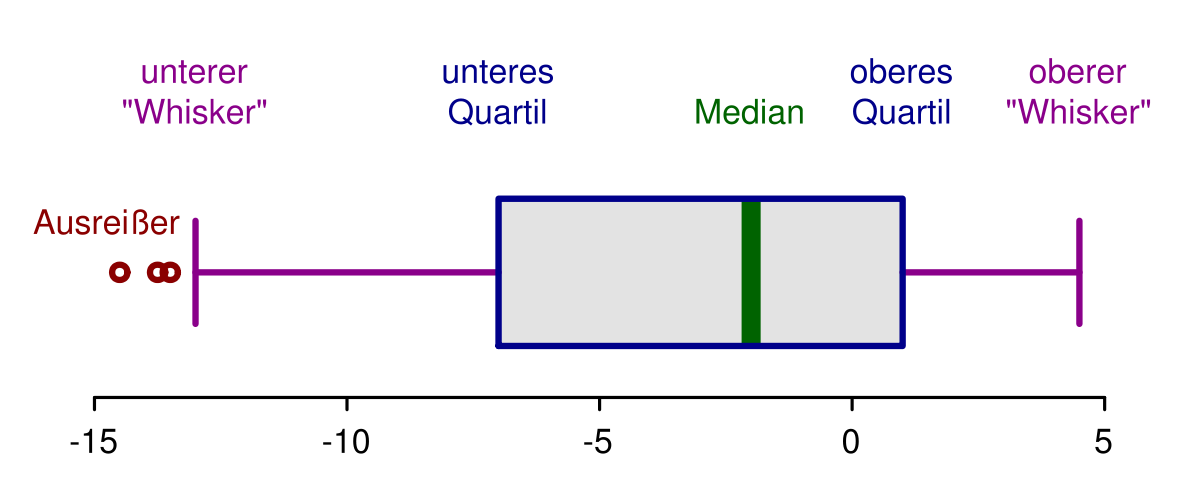
\includegraphics[width=0.9\textwidth]{Boxplot.png}
  \label{fig:Bild1}
\end{figure}
\section{Konzentrationsmaße}
Konzentrationsmaße messen, wie ungleich bzw. wie geballt konzentriert Messwerte der Merkmalsträger verteilt sind (relative Konzentrationsmaße). Mithilfe einer Lorenzkurve kann der Gini Koeffizient berechnet werden.
\subsection{Lorenzkurve}
Die Lorenzkurve ist eine graphische Darstellung der Verteilung.
Zum zeichnen einer Lorenzkurve geht man wie folgt vor:
\begin{enumerate}
    \item In einer sortierten Liste berechnet man zunächächt den kumulierten \textbf{Anteil an der Grundmenge} und erhält dadurch die x-Koordinaten:
    \begin{align*}
    u_k&=\frac{j}{n}
    \end{align*}
    \item Für die y-Koordinaten wird der kumulierte Anteil an der Merkmalssumme berechnet, wobei die Merkmalssumme berechnet wird durch:
    \begin{align*}
    Q=\sum_{i=1}^n x_i
    \end{align*}
    Die eigentliche Koordinate ergbit dich dann durch die Berechnung:
    \begin{align*}
    v_j=\frac{\sum_{i=1}^j x_i}{Q}
    \end{align*}
\end{enumerate}

\subsection{GiniKoeffizient-TODO}
\section{Zweidimensionale Urliste}
\subsection{Kontingenztabelle}
Über Kontingenztabellen können zwei Merkmale X und Y, z. B. ein ordinal- mit einem nominalskalierten, in Beziehung gebracht werden, um die Zusammenhänge der Merkmalsausprägungen strukturiert als Häufigkeiten h (siehe Klassenbildung) darstellen zu können. Des weiteren können folgende Häufigkeiten in einer Kontingenztabelle dargestellt werden:
\begin{itemize}
    \item Gemeinsame Häufigekit: Die Elemente in der Tabelle, die darstellen welche Stichproben auf beide Bedingungen zutreffen
    \item Absolute Randhäufigkeit: Summer alle absoluten Häufigkeiten in dieser Spalte/Zeile
    \item Bedingte (relative) Häufigkeit: Summer alle relativen Häufigkeiten in dieser Spalte/Zeile
\end{itemize}
$\Rightarrow$ Hierdurch kann einfach ein allgemeines Bild von Ursache und Wirkung erstellt werden.
\section{Streuungsdiagramm}
Ein Streuungsdiagramm wird verwendet wenn in einer Stichprobe viele verschiedene Ausprägungen bze. Merkmale vorhanden sind. Es werden dabei alle Merkmale mit einem Punkt in ein kartesisches Koordinatensystem eingetragen, wodurch sich eine Punktwolke ergibt. Man erhofft sich durch das Muster der Punkte im Streudiagramm Informationen über die Abhängigkeitsstruktur der beiden Merkmale zu erkennen, die durch die Koordinaten repräsentiert sind.
\newpage
\section{Kontingenzkoeffizient}
\section{Lineares Modell}
Ein lineares Modell wird verwendet, um einen bestimmten Erwartungswert Y\footnote{Regressand bzw. abhängige Variable} durch eine bestimmten lineare mit X\footnote{Regressor bzw. unabhängige Variable} Weise zu berechnen, die von einer gewissen Bedingungskonstellationen abhängt. Allgemein gilt:
\begin{eqnarray*}
y = f(x)
\end{eqnarray*}
Für einfache lineare Schätzungen (auch lineare Regression genannt) gilt:
\begin{eqnarray*}
yi = a + bxi + \epsilon i
\end{eqnarray*}
$\epsilon$: Fehler der Grundgesamtheit \newline

\subsection{Residuum}
Abweichung zwischen gegebenen Daten der Stichprobe und durch Modell geschätzten Werten
\begin{eqnarray*}Q(a,b)=\mathop{\sum ^{\infty }}\limits_{n=-\infty }{a}_{n}{(z-{z}_{0})}^{n},\end{eqnarray*}
(\={x}; \={y}) ist Datenschwerpunkt und liegt \textbf{immer} auf der Regrassionsgeraden!
\subsection{Fehlerquadratsumme}
TODO
\subsection{Varianz und Information}
Die Varianz ist ein Maß für die Streuung der Wahrscheinlichkeitsdichte um ihren Schwerpunkt. Sie wird definiert als die mittlere quadratische Abweichung einer reellen Zufallsvariablen von ihrem Erwartungswert.
\subsection{Determinationskoeffizient}
Der Determinationskoeffizient ist ein Maß für die Abweichungen der Vorhersagen eines Regressionsmodells von den empirischen Daten, also ein Maß für die Modellanpassung. Konkret entspricht dies dem Anteil der Variation der Modellvorhersagen, der sogenannten erklärten Summe der Abweichungsquadrate, an der Variation der beobachteten Werte der abhängigen Variablen, der sogenannten Gesamtsumme der Abweichungsquadrate. Er wird interpretiert als der durch die Regression erklärter Anteil der Varianz.
\newpage

\section{Taschenrechner}
\begin{enumerate}
    \item Häufigkeiten einschalten:
    $\Rightarrow$ SHIFT + SETUP + DOWN + 3 (Statistik)
    \item Statistik-Modus
    $\Rightarrow$ MENU + 6 + 1 (Variable)
    \item Daten und Häufigkeiten eingeben
    $\Rightarrow$ Abschluss der Dateneingabe durch AC
    \item Ergebnisse/Maßzahlen
    \item OPTN + 2 (1-Variab-Bereich)
\end{enumerate}
Dabei kann folgendes abgelesen werden:
\begin{table}[]
    \begin{tabular}{|r|l|}\hline
    \end{tabular}
\end{table}
\end{document}

